\subsection{KAGE} \label{background:kage}
KAGE \cite{kage} is an alignment-free genotyping tool for SNPs and short indels.
As opposed to alignment-based genotyping tools, KAGE relies on an alignment-free method where genotype-probabilities are computed using a statistical model.
These genotype-probabilities are supported by \textit{k}mer frequencies found in the input reads and previous knowledge of genetic variation and genotype information from thousands of individuals, produced by studies such as the 1000 Genomes Project \cite{1000_genomes_project}.
KAGE recently showed (2022) that its accuracy was on par with the best existing alignment-free genotyping tools while being an order of magnitude faster \cite{kage}.

KAGE is implemented in Python and relies heavily on the NumPy library for performance.
Its genotyping pipeline is split into two distinct programs: \textit{kmer\_mapper}, solving the \textit{partial} \textit{k}mer counting problem of counting \textit{k}mer frequencies for a predefined set of \textit{k}mers in the input reads, and \textit{kage}, which finally computes the genotype-probabilities using a statistical model.

\begin{figure}[H]
\begin{center}
\scalebox{1}{
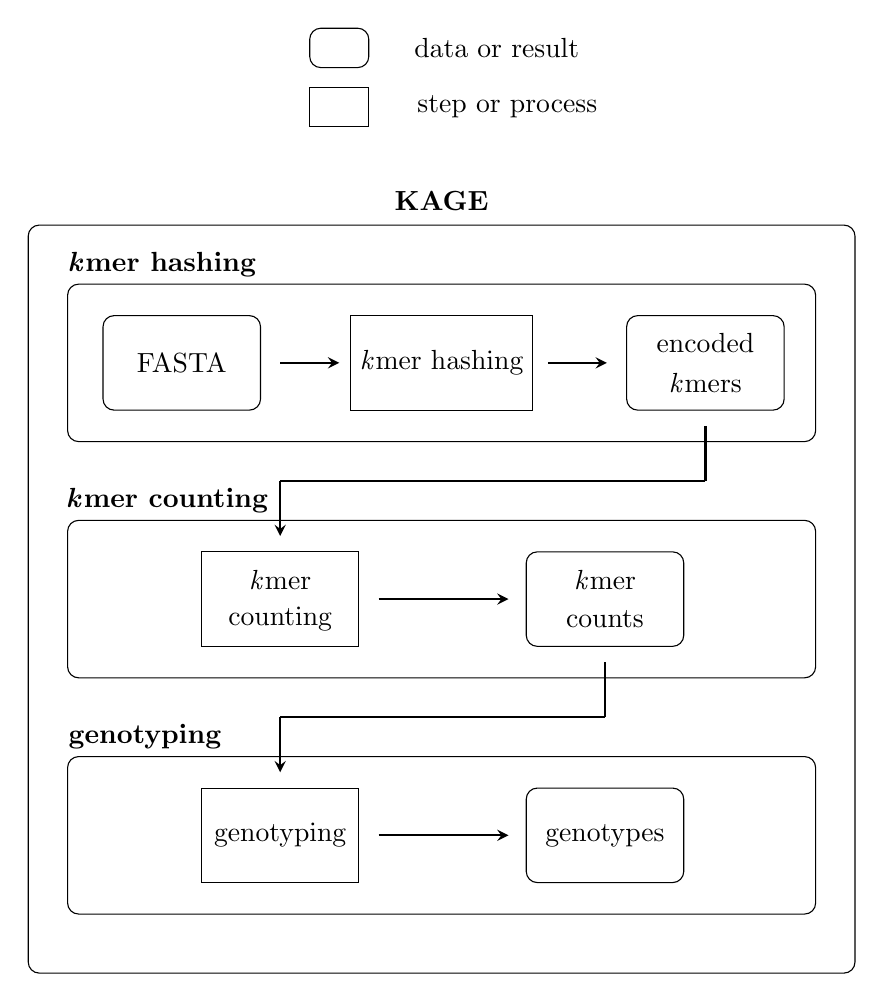
\begin{tikzpicture}
  % kmer hashing 
  \node at(-.25,1.25)[minimum width=2cm,minimum height=1.2cm](){\smaller\textbf{\textit{k}mer hashing}};
  \node at(0,0)[draw,minimum width=2cm,minimum height=1.2cm,rounded corners](){\smaller{FASTA}};
  \draw [thick,-stealth](1.25,0) -- (2,0);
  \node at(3.3,0)[draw,minimum width=2cm,minimum height=1.2cm](){\smaller{\textit{k}mer hashing}};
  \draw [thick,-stealth](4.65,0) -- (5.4,0);
  \node at(6.65,0)[draw,minimum width=2cm,minimum height=1.2cm,rounded corners]{};
  \node at(6.65,.25)[]{\smaller{encoded}};
  \node at(6.65,-.25)[]{\smaller{\textit{k}mers}};
  \node at(3.3,0)[draw,minimum width=9.5cm,minimum height=2cm,rounded corners](){};
  % arrows
  \draw [thick](6.65,-.8) -- (6.65,-1.5);
  \draw [thick](6.65,-1.5) -- (1.25,-1.5);
  \draw [thick,-stealth](1.25,-1.5) -- (1.25,-2.2);
  % kmer counting 
  \node at(-.185,-1.75)[minimum width=2cm,minimum height=1.2cm](){\smaller\textbf{\textit{k}mer counting}};
  \node at(3.3,-3)[draw,minimum width=9.5cm,minimum height=2cm,rounded corners](){};
  \node at(1.25,-3)[draw,minimum width=2cm,minimum height=1.2cm]{};
  \node at(1.25,-2.75)[]{\smaller{\textit{k}mer}};
  \node at(1.25,-3.25)[]{\smaller{counting}};
  \draw [thick,-stealth](2.5,-3) -- (4.15,-3);
  \node at(5.375,-3)[draw,minimum width=2cm,minimum height=1.2cm,rounded corners]{};
  \node at(5.375,-2.75)[]{\smaller{\textit{k}mer}};
  \node at(5.375,-3.25)[]{\smaller{counts}};
  % arrows
  \draw [thick](5.375,-3.8) -- (5.375,-4.5);
  \draw [thick](5.375,-4.5) -- (1.25,-4.5);
  \draw [thick,-stealth](1.25,-4.5) -- (1.25,-5.2);
  % genotyping
  \node at(-.465,-4.75)[minimum width=2cm,minimum height=1.2cm](){\smaller\textbf{genotyping}};
  \node at(3.3,-6)[draw,minimum width=9.5cm,minimum height=2cm,rounded corners](){};
  \node at(1.25,-6)[draw,minimum width=2cm,minimum height=1.2cm](){\smaller{genotyping}};
  \draw [thick,-stealth](2.5,-6) -- (4.15,-6);
  \node at(5.375,-6)[draw,minimum width=2cm,minimum height=1.2cm,rounded corners](){\smaller{genotypes}};
  % KAGE
  \node at(3.3,2.05)[minimum width=2cm,minimum height=1.2cm](){\smaller\textbf{KAGE}};
  \node at(3.3,-3)[draw,minimum width=10.5cm,minimum height=9.5cm,rounded corners](){};
  % Hints 
  \node at(2,4)[draw,minimum width=.75cm,minimum height=.5cm,rounded corners](){};
  \node at(4,4)[](){data or result};
  \node at(2,3.25)[draw,minimum width=.75cm,minimum height=.5cm](){};
  \node at(4.135,3.25)[](){step or process};
\end{tikzpicture}
}
\caption{
  A simplified illustration of how the KAGE genotyping pipeline works.
  The two top most rows, going from an input FASTA file to \textit{k}mer counts, are implemented as an individual piece of software.
  Three important parts of the pipeline are shown as distinct processes in the illustration: 
  1) \textbf{\textit{k}mer hashing}, which refers to the process of 2-bit encoding input reads from the fasta file and extracting - \textit{hashing} - all valid \textit{k}mers from those reads, 
  2) \textbf{\textit{k}mer counting}, which refers to the process of \textit{partial k}mer counting - counting the observed frequencies of a predefined set of \textit{k}mers in the input reads, and 
  3) \textbf{genotyping}, which refers to the process of computing the final genotype-probabilities.
}
\label{background:kage:figures:pipeline}
\end{center}
\end{figure}

